\setcounter{mtc}{5} %indique le num�ro r�el du chapitre, pour la mini table des mati�res
\chapter{Cadre du projet}
\minitoc %insert la minitoc
\graphicspath{{Chapitre1/figures/}}
%==============================================================================
\pagestyle{fancy}
\fancyhf{}
\fancyhead[R]{\bfseries\rightmark}
\fancyfoot[R]{\thepage}
\renewcommand{\headrulewidth}{0.5pt}
\renewcommand{\footrulewidth}{0pt}
\renewcommand{\chaptermark}[1]{\markboth{\MakeUppercase{\chaptername~\thechapter. #1 }}{}}
\renewcommand{\sectionmark}[1]{\markright{\thechapter.\thesection~ #1}}

\begin{spacing}{1.2}
%==============================================================================
\section*{Introduction}
Ce premier chapitre a pour objectif de situer le projet dans son cadre général. Nous présenterons donc l’organisme d’accueil, son historique et ses secteurs d'activité. Nous enchaînerons sur les problématiques et les solutions proposées, la méthodologie de travail adoptée et nous achèverons par une présentation de quelques concepts de base et étude de l’existant.
\vspace{-3mm}
\section{Présentation de l'organisme d’accueil: Konvergence B\&T}
\subsection{Présentation générale}
Basée à Paris, Konvergence a été fondée en janvier 1987. Société par actions simplifiées, à associé unique, elle compte 65 salariés. L'effectif est divisé en trois départements majeurs: R\&D, Services et Consulting. Grâce à son personnel très actif, l’entreprise a réussi à imposer sa place parmi les leaders mondiaux de son marché avec un chiffre d'affaires de 31 000,00 € pour l'année 2006 et à se développer également au niveau international avec l’ouverture d’une filiale aux Etats-Unis et en Tunisie. Le total de son bilan a augmenté de 99,00 \% entre 2005 et 2006.\\

À l'origine, intégrateur de solutions de mesure de la performance financière des solutions Oracle Hyperion, Konvergence a conçu initialement le logiciel Shuttle comme un Add-On\footnote{extension à un autre logiciel} renforçant la plateforme Oracle Hyperion Essbase. Au fil du temps, Shuttle est devenu une plateforme à part entière\cite{shuttle}, concurrente de celle d'Oracle. De ce fait, Konvergence a décidé de faire une spin-off et rendre le Shuttle indépendant et quitter l'activité d'intégration des solutions Hyperion Essbase. 
Aujourd'hui, la boite est spécialisée dans l’édition de logiciels applicatifs et l'intégration des ses propres solutions BI/EPM.

\subsection{Secteurs d'activité}
Konvergence est l’éditeur de la solution Shuttle, une solution dédiée au pilotage de la décision dans les domaines de la performance financière et opérationnelle, de la gestion des risques et de la gouvernance. Elle intègre au sein d’une seule plateforme des fonctionnalités de collecte de données, de gestion de bases de données, de restitution, d'aide à la décision, de Disclosure Management et de Reporting  [annexe A.1]. Cette solution est déployée à l’international et rencontre un succès croissant auprès de ses clients. Elle offre une plateforme évolutive avec une efficacité opérationnelle permettant de créer dynamiquement des applications intégrées d'EPM, de BI, de BAM et de GRC [annexe A.1]. 
La figure I.1 montre les clients de Konvergence par domaine d'application.
\begin{figure}[H]\centering 
	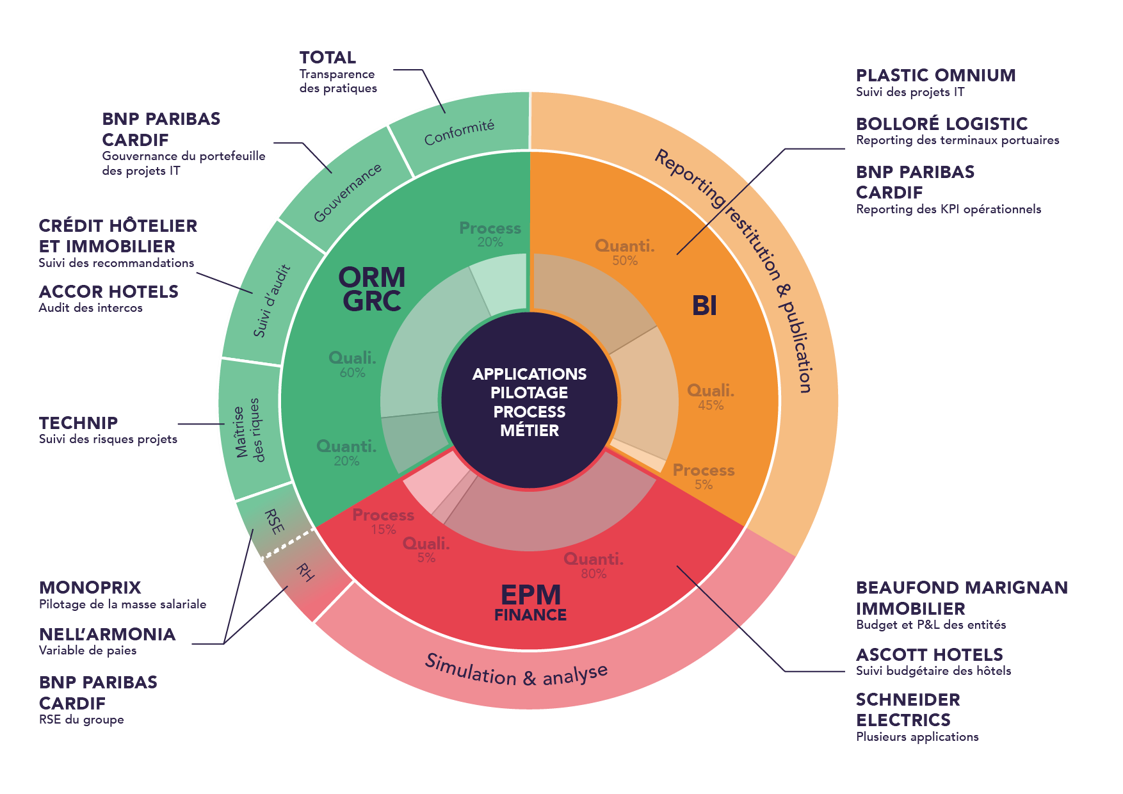
\includegraphics[scale=0.5]{solutions}
	\caption{Clients Shuttle par domaine}\cite{intern}
	\label{fig:fig2}
\end{figure}

%La figure A.1 présente l'architecture applicative de la solution Shuttle.
\vspace{-3mm}
\section{Présentation des projets}
\subsection{Intégration continue et tests automatiques IFRS16}
\subsubsection{Contexte et problématiques}

Les normes IFRS ont pour objectif d’harmoniser la présentation des états financiers des entreprises.
L'IASB a publié le 13 janvier 2016 la norme IFRS 16\cite{ifrs16}. 
Très brièvement, IFRS 16 est un standard de finance qui désormais impose la comptabilisation au bilan du preneur de tous les contrats de location.
Nombreuses entreprises, indépendamment de leur secteur d’activité, font le choix d’intégrer dans leurs systèmes d’information des outils informatiques permettant la mise en œuvre de cette norme.

Conciente de cet enjeu, Konvergence édite une application nommée "K-IFRS16", qui offre la facilité de gestion et de suivi d’un volume important de contrats de locations établis conformément à la norme IFRS 16. Cette application est basée sur les solutions propriétaires de l’entreprise : la plateforme Shuttle. 

Konvergence a mis en oeuvre une équipe dédiée à l'édition de l'outil K-IFRS16. Des consultants, fonctionnels, experts comptables, des développeurs et des testeurs ont pour mission de développer et assurer la livraison d'un produit de qualité à leur clients.

Toutefois, les tests de cet outil sont faites manuellement, donnant plus de chance à l'erreur humaine et prennant beaucoup de temps et effort.

Le processus de développement et test de l'application est comme suit : 
\begin{itemize}
\setlength\itemsep{0em}
    \item Un consultant fonctionnel demande à l'équipe de développeurs d'ajouter une fonctionnalité en les expliquant le besoin.
    \item Les développeurs implémentent le besoin, rajoutent des tests unitaires et livrent la nouvelle application aux testeurs.
    \item Les testeurs font appelles aux consultants pour demander les scénarios de tests possibles et les résultats attendus.
    \item Les consultants décrivent les scénarios et fournissent les résultats attendus sous forme de fichiers CSV.
    \item Les testeurs, après avoir exécuté les scénarios à la main, comparent les résultats case par case. En cas d'erreur, ils appellent les fonctionnels et les développeurs pour investiguer les anomalies.
\end{itemize}
De plus, la livraison de l'application était manuelle. Un processus long demeurant de plus en plus difficile, avec la multitude de version et configuration.
\subsubsection{Solution proposée : IFRS16 CI/CD Pipelines}
Dans ce cadre, nous avons mis en place trois chaines d'intégration et livraison continues pour les différentes versions de l'application K-IFRS16. Partant de l'outil de gestion de code source, un pipeline IFRS16, construit le projet, exécute les tests unitaires, déploie les artefacts, prépare un environnement Cloud de tests et exécute les différents scénarios de tests de non-regréssion. Nous verrons plus en détails ces pipelines dans le chapitre qui suit. 
\subsection{Automatisation du processus de Benchmark Tests}
\subsubsection{Contexte et problématiques}
Shuttle est un outil de BI/EPM puissant et très flexible\cite{intern}. Il offre la compatibilité avec une large gamme de bases de données relationnelles et tourne sur les trois systèmes d'exploitation les plus utilisés: Windows, Mac et Linux. Étant données les préférences et les spécificités de chaque client, le bon fonctionnement, la non-régression, les performances et la haute disponibilité de la plateforme sont des contraintes très importantes. 
Pour assurer ces dernières, des tests de performance, "Benchmark Tests", sont nécessaires sur les différents environnements offerts. 
Le processus de Benchmark tests était manuel. L'ingénieur QA commence par la création et le déploiement de l'environnement, ensuite il lance les tests, puis il enregistre les résultats sous forme de fichiers CSV pour les synthétiser enfin dans une feuille Excel. Cette méthode est assez lente et nécessite beaucoup de concentration. De plus, le reporting étant statique, ceci rend l'investigation des résultats très difficile. 
C'est dans ce contexte que le projet de "Bench Tests Pipeline" a été nécessaire.
\subsubsection{Solution proposée : Bench Tests Pipeline}
Nous allons mettre en place un mécanisme automatique de construction d'environnement Shuttle, de lancement des tests de performance et de reporting des résultats. Cette solution offre la flexibilité dans les choix des services et bases de données à déployer dans l'environnement cloud, la durée des tests et différents indicateurs et graphiques pour le reporting.
\section{Méthodologie de travail : Scrum}
\subsection{Méthodologie agile}
En février 2001, aux Etats Unis, 17 spécialistes du développement logiciel se sont réunis pour débattre du thème unificateur de leurs méthodes respectives, dites méthodes agiles. De cette réunion a émergé le Manifeste Agile considéré comme la définition canonique du développement Agile et de ses principes sous-jacents. 

Durant notre projet, nous avons intégré principalement l'équipe R\&D qui applique l'agilité depuis 3 ans.
Constituée de 12 personnes dont un Release Manager, un ingénieur DevOps, huit développeurs, un architecte et un Product Owner, nous avons assuré la partie DevOps au sein de cette équipe. Nous avons fait le relais entre les différentes équipes de la boite en travaillant également à la fois avec l'équipe de développement de la plateforme, l'équipe Apps qui développent les applications en utilisant le Shuttle, l'équipe Ops et l'équipe IT. Le but était d'éliminer les silos et permettre une meilleure intéraction dans la boite. Nous avons bien entendu adopté une méthode agile pour le pilotage de nos projets, c'est la méthode Scrum.

Cette méthodologie offre une meilleure adaptabilité, visibilité et gestion des risques. Elle se caractérise par un modèle de développement itératif, où les exigences et les solutions évoluent grâce à la collaboration entre des équipes interfonctionnelles, un processus de gestion de projet qui encourage une inspection et une adaptation fréquentes, l'auto-organisation et la responsabilisation, un ensemble de valeurs et de bonnes pratiques et une approche métier alignant le développement sur les besoins des clients et les objectifs de l'entreprise. Elle fait référence à tout processus de développement aligné sur les concepts du Manifeste Agile [annexe B]\cite{manifesto}.
\subsection{Scrum}
Scrum, un cadre de processus léger pour le développement agile, est le plus souvent utilisé pour la gestion des projets complexes. Il se distingue des autres processus agiles par des concepts et des pratiques spécifiques, divisés en trois catégories : Rôles, Artefacts et Boîtes de temps. Cette méthodologie a comme objectif d’augmenter la productivité et la qualité des livrables et de réduire le délai d'obtention des avantages par rapport aux processus "cascade" classiques. Elle permet aux équipes de s'adapter facilement à l’évolution rapide des exigences et de répondre aux changements d’objectifs des métiers qui sont en constante évolution.
La construction du produit se fait en plusieurs itérations d'une durée de 2 à 4 semaines nommées "Sprint". Durant chacune de ces itérations, une partie du produit nommée "Incrément" est réalisée en se basant sur ce qui précède et est livrée à la fin du sprint. La figure I.2 explique le déroulement du processus Scrum.
\begin{figure}[!ht]\centering
\includegraphics[scale=0.22]{"scrum".png}
\caption{Cycle de vie d'un processus Scrum \cite{scrum}}
\label{fig:fig1}
\end{figure}
\FloatBarrier
\textbf{Rôles:}
\begin{itemize}
\setlength\itemsep{0em}
    \item[--] Scrum Master : Le gardien du processus. Responsable du bon déroulement du processus, de l'élimination des obstacles et de l'organisation des réunions critiques.
    \item[--] Product Owner : Le gardien des exigences. La « source unique de vérité » en ce qui concerne les exigences et l'ordre de mise en œuvre planifié. C'est l'interface entre l'entreprise, les clients et leurs besoins liés aux produits d'un côté, et l'équipe de l'autre.
    \item[--] Equipe Scrum : Une équipe auto-organisée et interfonctionnelle, comptant idéalement entre cinq et neuf personnes, qui effectue le travail de développement et de test. Elle a également le pouvoir de prendre des décisions sur la façon d'effectuer le travail.
\end{itemize}

\textbf{Product Backlog : }
Une liste ordonnée de tout ce qui doit être fait, les exigences fonctionnelles et non fonctionnelles, sous forme de user story qui remplace les artefacts de spécification des exigences traditionnelles.

\textbf{Réunions : }
\begin{itemize}
\setlength\itemsep{0em}
\item[--] Planification du sprint : Se déroule au début de chaque sprint, dans le but de mettre en place une liste d'éléments prioritaires du Product Backlog à réaliser au cours du sprint.   
\item[--] Revue de sprint: Présenter, à la fin du sprint, le travail accompli par l’équipe lors du dernier sprint.
\item[--] Rétrospective de sprint : A pour objectif de découvrir ce qui a bien fonctionné et ce qui n'a pas fonctionné lors du dernier sprint et comment s'améliorer.
\item[--] Mêlée quotidienne : Se tient tous les jours et se fait debout pour que la réunion soit courte et précise. Elle permet aux membres de l’équipe de s'informer mutuellement.
\end{itemize}
\subsection{Équipe et rôles}
Durant notre stage, nous avons intégré l’équipe R\&D chez Konvergence. L’équipe compte 12 personnes. Elle se décompose en un ensemble des sous-équipes interfonctionnelles qui collaborent entre elles. Nous allons travailler avec toutes ces équipes, ainsi que d'autres, en faisant le relais entre les Devs, l'IT et l'Ops. Nous allons collaborer notamment avec la Release Manager pour assurer les tests automatiques, l'intégration et la livraison continues.
\begin{table}[ht]
	\centering
	\caption{Rôle et membres}
	\footnotesize
	\begin{tabularx}{\textwidth}{|X|X|}
          \hline
          {\textbf{Rôle}}
          & 
          {\textbf{Membres}} 
          \\
          \hline
          Release Manager & Mme. Valérie NOYER \\    \hline
          Scrum Master & Mr. Hamza NOURI \\          \hline
          Product Owner & Mr. Nicolas DERYCKE \\          \hline
          Operations & Mr. Olivier ROCHON \\          \hline
          IT Infrastructure  & Mr. Paul LECLERC \\          \hline
          Testeurs & Mr. Nader KASRI \\          \hline
          Stagiaire CI/CD DevOps & Rafik BAHRI \\          \hline
          Dev & Les développeurs \\          \hline
        \end{tabularx}
	\label{tab:exple}
\end{table}
\FloatBarrier
Nous avons divisé nos travaux en Sprints par sujet. La figure I.3 explique le déroulement de notre stage. 
\begin{figure}[H]\centering
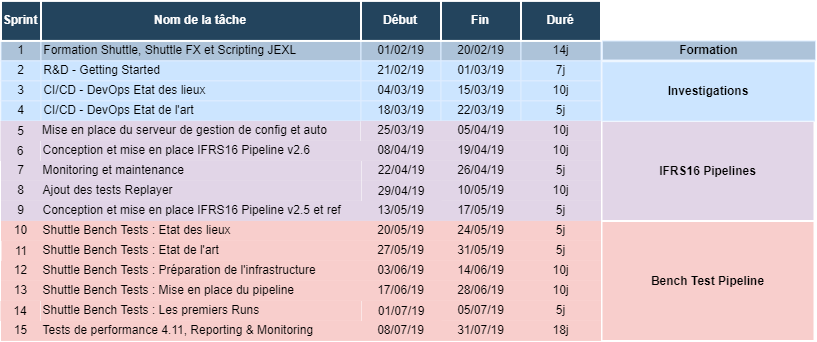
\includegraphics[scale=0.5]{Chapitre2/figures/gant.png}
\caption{La liste des sprints}
\label{fig:fig1}
\end{figure}
\FloatBarrier
Nous allons aborder, dans le paragraphe qui suit, quelques concepts de base ainsi que l'état des lieux que nous avons fait.
\section{Concepts de base et étude de l’existant}
\subsection{CI/CD et DevOps}
\textbf{CI (Continuous Integration)} : La pratique utilisée en Génie Logiciel permettant d'intégrer plusieurs fois pendant la journée les changements effectués sur le code du projet, et ceci d'une manière automatique qui déclenche un build et les tests, afin de détecter les erreurs et les régressions au plus tôt possible. 

\textbf{CD (Continuous Delivery/Deployment)} : L'acronyme CD peut etre utilisé pour décrire l'un des termes : 
\begin{itemize}
    \item Continuous Delivery : La livraison continue est l'approche dans laquelle les équipes produisent des logiciels dans des cycles courts, ce qui permet de le mettre à disposition à n’importe quel moment. Le but est de construire, tester et diffuser un logiciel plus rapidement.
    \item Continuous Deploiment : Le déploiement continué est la stratégie de développement où toute validation de code qui réussit le cycle de build et test automatiques est transférée dans l'environnement de production, propulsant ainsi les modifications vers les utilisateurs finaux du logiciel.
\end{itemize}
\begin{figure}[H]\centering
\includegraphics[scale=0.3]{"devops-cycle-without-deployement".png}
\caption{Process d'intégration et livraison continue existant du Shuttle}
\label{fig:fig2}
\end{figure}

\textbf{DevOps (Development \& Operations)} : DevOps est un ensemble de pratiques qui met l'accent sur la collaboration et la communication entre les développeurs de logiciels et les professionnels des opérations informatiques, en automatisant le processus de livraison de logiciels et les changements d'infrastructure.

\begin{figure}[H]\centering
\includegraphics[scale=0.25]{"devops".png}
\caption{Cycle DevOps}
\label{fig:fig3}
\end{figure}
Le cycle de DevOps se décompose comme suit : 
\begin{enumerate}
\setlength\itemsep{0em}
      \item Plan : la planification des différentes taches, tickets et autres jalons
      \item Create : la concrétisation des taches planifiées
      \item Verify : le test et l'acceptance des développements effectués
      \item Package : la construction des artefacts prêts à la livraison
      \item Release : la livraison des artefacts après tests
      \item Configure : la configuration et le déploiement des produits
      \item Monitor : la surveillance des produits ainsi déployés
\end{enumerate}

\subsection{Étude de l’existant}
\textbf{La palteforme} : Shuttle est une solution logicielle unifiée et collaborative, dédiée au pilotage de la décision Son modèle collaboratif est renforcé par sa capacité à gérer tout processus et à aider l'entreprise à progresser vers l'excellence opérationnelle. La figure I.4 décrit l'architecture technique de la solution Shuttle.
\begin{figure}[H]\centering
\includegraphics[scale=0.4]{"shuttle arch app".PNG}
\caption{Architecture technique de la solution Shuttle}
\label{fig:fig4}
\end{figure}
\FloatBarrier
Elle est composée du :
\begin{itemize}
    \setlength\itemsep{0em}
    \item[--] Référentiel : constitué des métadonnées dont l’application a besoin pour fonctionner.
    \item[--] Des règles de calcul : Shuttle possède  un moteur de calcul afin de centraliser ces règles.
    \item[--] D’un processus métier digitalisé à l’aide de Shuttle.
    \item[--] D’un dispositif de sécurité d’accès aux métadonnées, aux données et aux objets applicatifs.
    \item[--] D’un moteur de stockage de données propriétaire ShuttleDB : une technologie unique hybride, qui combine à la fois les caractéristiques OLAP [annexe A.3] et OLTP [annexe A.4].
    \item[--] D’applications client qui offrent des interfaces permettant de collecter de l’information auprès de l’utilisateur et des rapports qui présentent le résultat de la restitution de ces données.
\end{itemize}

\FloatBarrier
\textbf {Le serveur} : C'est la partie Backend de la plateforme. Le serveur Shuttle est l'outil permettant la conception des applications, la modélisation des données dans des cubes multi-dimesionels ainsi que la construction des IHM. Il permet également aux administrateurs de gérer les droits d'accès, la sécurité des applications et des données. 

\textbf {Le client} : Shuttle FX est le nom du client de la plateforme Shuttle. C'est une application Desktop basée sur la plateforme JavaFX. D'où le nom ShuttleFX. Le client permet la consultation des applications Shuttle et la manipulation des données. 

\textbf {Les plugins} : La plateforme permet le développement des plugins pour étendre la partie Serveur mais aussi la partie cliente. Le plugin Recorder/Replayer, est le plus connu et utilisé en interne dans la boite. Ce dernier offre la possibilité d'enregistrer (Recorder) et rejouer (Replayer) un scenraio contenant une séquence d'actions déterminée par l'ingénieur qualité. Nous allons prendre avantage de ce plugin pour concevoir des tests automatiques dans le chapitre prochain.

\textbf{L'AddIn Office} : Konvergence offre parmi sa gamme de produits, une extension au produit Excel de Microsoft. Cet AddIn permet l'interaction avec des applications Shuttle à travers MS Excel, en permettant plus de flexibilité à l'utilisateur final. 

\textbf{La chaine d'intégration et livraison continues} : Konvergence utilise une boite à outils riche pour la livraison de son logiciel principal, le Shuttle. 
Le tableau ci-dessous présente les outils et technologies utilisés pour la construction de la chaine existante. 
\begin{table}[ht]
	\centering
	\caption{La boite à outils}
	\footnotesize
	\begin{tabularx}{\textwidth}{|p{3.3cm}|p{3.3cm}|X|}
          \hline
          {\textbf{Besoin}}
          & 
          {\textbf{Outil}} 
          & 
          {\textbf{Description}} 
          \\
          \hline
          Gestion de code source & Subversion (SVN) & Centralisé, model client serveur \\    \hline
          Gestion de dépendances & Maven  & Gestion efficace des dépendances et automatisations des constructions des projets Java \\    
          \hline
          Gestion des artefacts & JFrog Artifactory & Artifact repository, indépendant de la téchnologie et hautement disponible  \\          \hline
          Qualité de code & SonarQube & Analyse et mesure de qualité de code en continu \\          \hline
          Intégration Continue & Jenkins & Open source, très flexible et extensible. Plus de 1000 plugin et communauté très active \\          \hline
        \end{tabularx}
	\label{tab:exple}
\end{table}
\FloatBarrier

\FloatBarrier

La figure I.7 représente le pipeline CI/CD existant de la plateforme. 
\begin{figure}[H]\centering
\rotatebox[origin=c]{-90}{\includegraphics[height=15cm,width=23cm]{"shuttle-new-pipeline".png}}
\caption{Pipeline CI/CD principal de produits Shuttle}
\label{fig:fig5}
\end{figure}

Le tableau suivant explique brièvement le rôle de chaque job \footnote{c'est une tâche automatisée ou une séquence d'instruction qu'on définit sur Jenkins dans sa version 1.0.} du processus du build. 

\begin{table}[ht]
	\centering
	\caption{Description des jobs}
	\footnotesize
	\begin{tabularx}{\textwidth}{|p{3.3cm}|X|}
          \hline
          {\textbf{Job}}
          & 
          {\textbf{Description}} 
          \\
          \hline
          {\textbf{SHUTTLE-NewBuild}} & La mise à jour du code source à partir de Subversion, ensuite la construction du projet avec Maven et le déploiement des artefacts produits dans l'Artifactory\\    \hline
         {\textbf{DEPLOY-*}} &  Le dépoiement du serveur et client Shuttle sur les différents systèmes d'exploitations supportés par la plateforme \\    
          \hline
          {\textbf{UI-Test-NomBrowser-NomDB}} & Lancement des tests d'interface utilisateur sur les différents navigateurs et les différentes base de données supportés   \\          \hline
          {\textbf{Replayer-*}} & Lancement des scenarios de tests enregistrer par le plugin Recorder en attaquant à chaque fois une base de données supportée par la plateforme \\          \hline
          {\textbf{SHUTTLE-Sonar}} & Analyses statiques du code et publication des résultats dans Sonar. \\          \hline
        \end{tabularx}
	\label{tab:exple}
\end{table}

\FloatBarrier

\FloatBarrier

Toutefois, cette chaine ne permet pas la livraison des applications basées sur le Shuttle telle que celle la plus dynamique, K-IFRS16. Nous aborderons ce sujet dans le chapitre qui suit, qui couvrira, l'analyse des besoins, la conception et l'implémentation des pipelines IFRS16.

\FloatBarrier
\section*{Conclusion}

Ce premier chapitre nous a permis de présenter l'organisme d’accueil, l'entreprise Konvergence B\&T, les projets qui ont fait l’objet  de notre stage. Nous allons évoquer dès à présent  les problématiques que nous avons traitées et les solutions proposées. Ce  sera également l’occasion de présenter les concepts CI/CD, DevOps, Pipeline as Code, Infra as Code que nous allons mis en oeuvre durant nos travaux.\\

Nous consacrerons le chapitre suivant à détailler les chaines d'intégration et livraison continues de l'application IFRS16 ;  des besoins techniques et fonctionnels qu’elles doit remplir,  des phases de conception, de mise en place et de configuration pour les différentes versions de l'application. 



%==============================================================================
\end{spacing}
